\documentclass[11pt]{article}
\usepackage[utf8]{inputenc}
\usepackage[spanish]{babel}
\usepackage[margin=2.3cm]{geometry}
\usepackage{amsmath,amssymb}
\usepackage{enumitem}
\usepackage{tcolorbox}
\tcbuselibrary{skins,breakable}
\usepackage{pgfplots}
\pgfplotsset{compat=1.18}
\usepackage{tikz}
\usepackage{graphicx}
\usepackage{array}
\usepackage[hidelinks]{hyperref}

% Notación española opcional (descomenta si quieres \sen en lugar de \sin)
% \DeclareMathOperator{\sen}{sen}
% \DeclareMathOperator{\tg}{tg}
% \DeclareMathOperator{\ctg}{ctg}

\newtcolorbox{sol}{colback=blue!5,colframe=blue!50!black,title=Solución paso a paso,breakable}
\newtcolorbox{teo}{colback=orange!8,colframe=orange!70!black,title=Teoría,breakable}
\newtcolorbox{nota}{colback=green!5,colframe=green!50!black,title=Idea clave,breakable}
\newtcolorbox{tip}{colback=yellow!10,colframe=yellow!60!black,title=Consejo,breakable}
\newtcolorbox{resp}{colback=red!5,colframe=red!50!black,title=Respuesta,breakable}
\newtcolorbox{reg}{colback=red!5,colframe=red!60!black,title=Regla,breakable}
\newtcolorbox{paso}[1]{colback=gray!5,colframe=gray!50!black,title={#1},breakable}

\graphicspath{{../images/}{images/}}
\newcommand{\sen}{\operatorname{sen}}

% babel spanish activa < y > y rompe TikZ/pgfplots (->, >=stealth)
\AtBeginDocument{\shorthandoff{<>}}

\usepackage{pdfpages}
\usepackage{fancyhdr}

% Numeración global: arriba a la derecha, para no chocar con la
% numeración propia (abajo, centrada) que cada parte ya trae impresa.
\fancypagestyle{global}{%
  \fancyhf{}%
  \renewcommand{\headrulewidth}{0pt}%
  \fancyhead[R]{\footnotesize\thepage}%
}
\pagestyle{global}
\setcounter{secnumdepth}{0}  % partes sin numerar: el índice ya las ordena

\begin{document}

%======================= PORTADA =======================
\begin{titlepage}
\thispagestyle{empty}
\centering
\vspace*{4.5cm}

{\Huge\bfseries Solucionario}\\[0.6em]
{\LARGE Unidad 1 --- Funciones}\\[2.2cm]

{\large Matemática General}\\[3.5cm]

\rule{0.55\textwidth}{0.4pt}\\[1em]
{\large Ejercicios seleccionados de}\\[0.4em]
{\large Stewart, Redlin y Watson}\\[0.3em]
{\large\itshape Precálculo. Matemáticas para el cálculo}\\[0.3em]
{\large 7.ª edición}\\[1em]
\rule{0.55\textwidth}{0.4pt}\\[2.5cm]

{\large 165 ejercicios resueltos --- 15 por sección}

\vfill
\end{titlepage}

%======================= ÍNDICE =======================
\clearpage
\pagenumbering{roman}
\setcounter{page}{1}

\tableofcontents

\vspace{2em}
\noindent\rule{\textwidth}{0.4pt}
\vspace{0.8em}

\small
\noindent Cada ejercicio se reproduce \emph{textual} del libro antes de resolverse. Las soluciones
usan únicamente los métodos que el propio libro presenta hasta la sección correspondiente:
sin derivadas, sin límites y sin herramientas de capítulos posteriores.

\medskip
Las secciones §1.8, §3.6 y §3.7 cubren temas del programa del curso (valor absoluto,
asíntotas y signo de una función) que el capítulo 2 del libro no trata.

\medskip
Esta edición del libro no incluye apéndice de respuestas: cada resultado fue derivado
y verificado de forma independiente.
\normalsize

%======================= PARTES =======================
\clearpage
\pagenumbering{arabic}
\setcounter{page}{1}

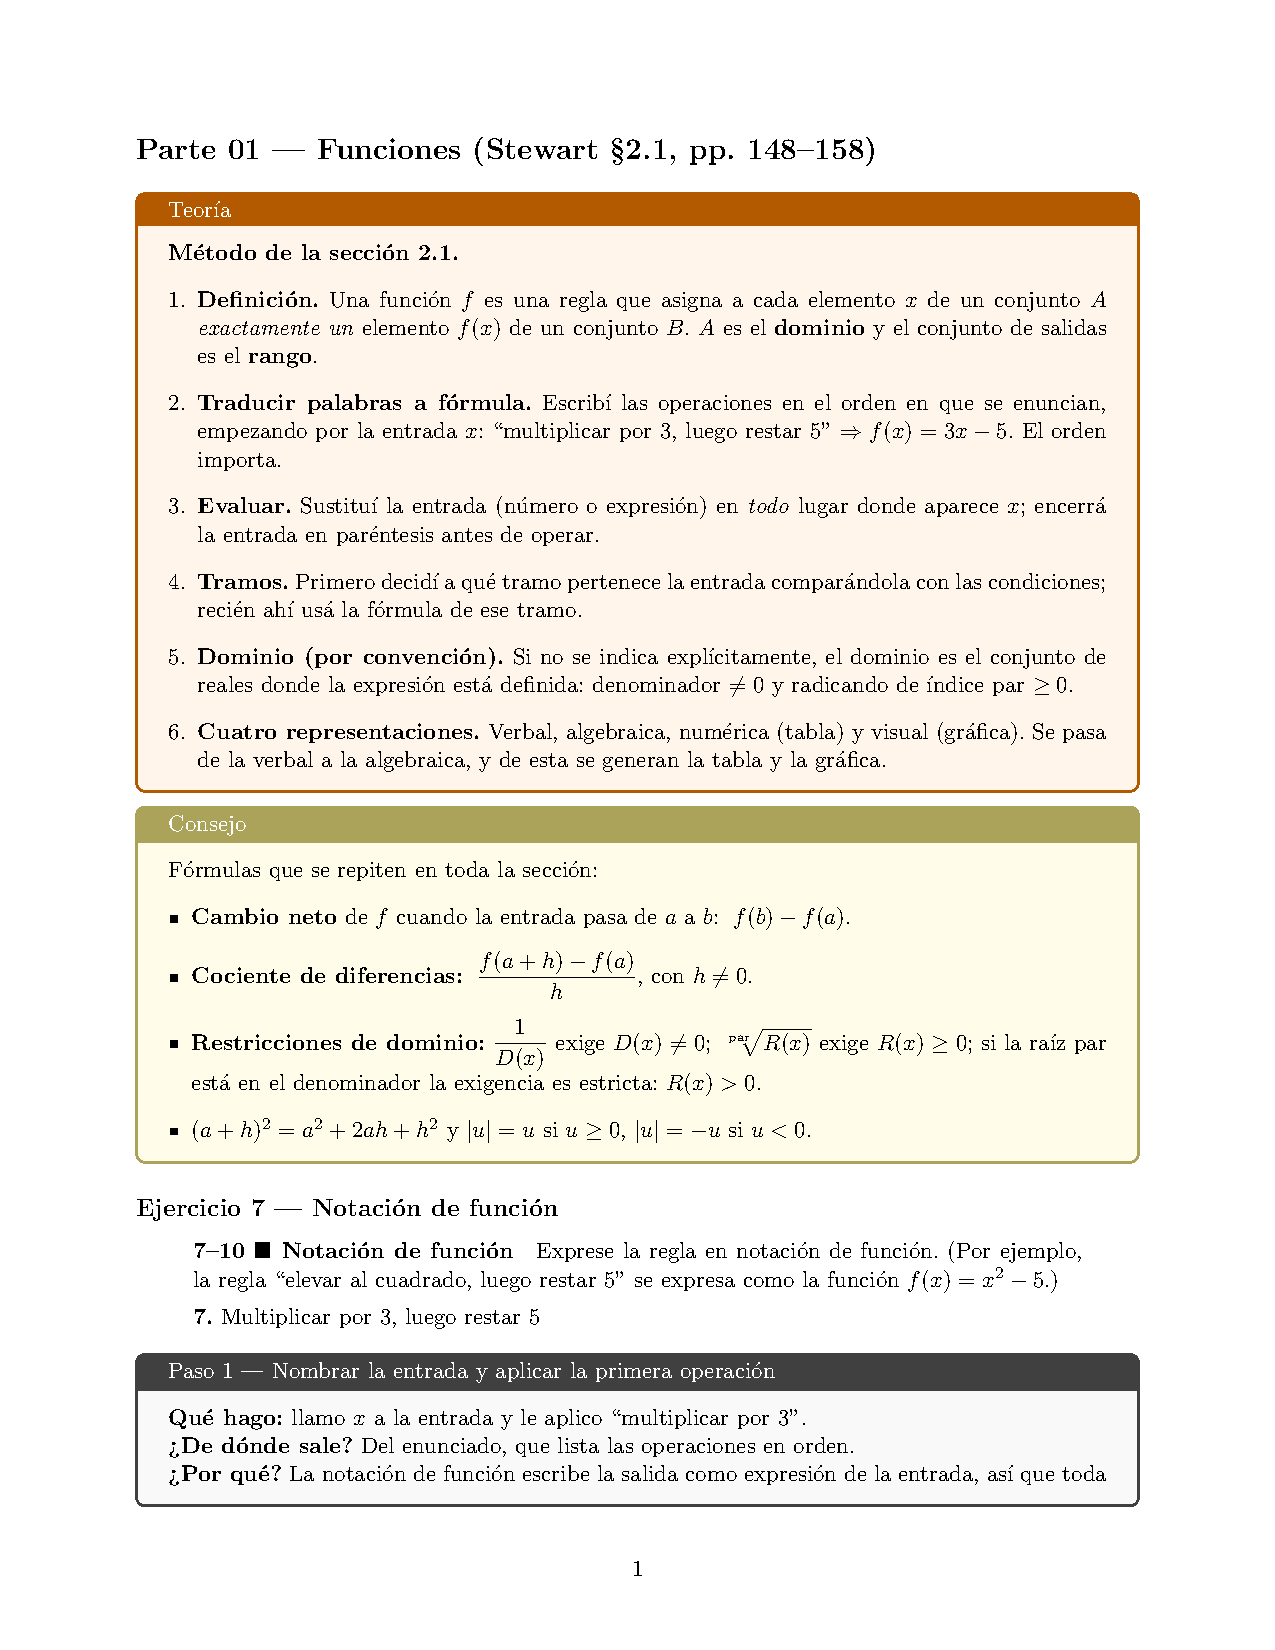
\includepdf[pages=-,pagecommand={\thispagestyle{global}},
  addtotoc={1,section,1,Parte 01 --- §2.1 Funciones,p01}]{../pdf/parte01_funciones.pdf}
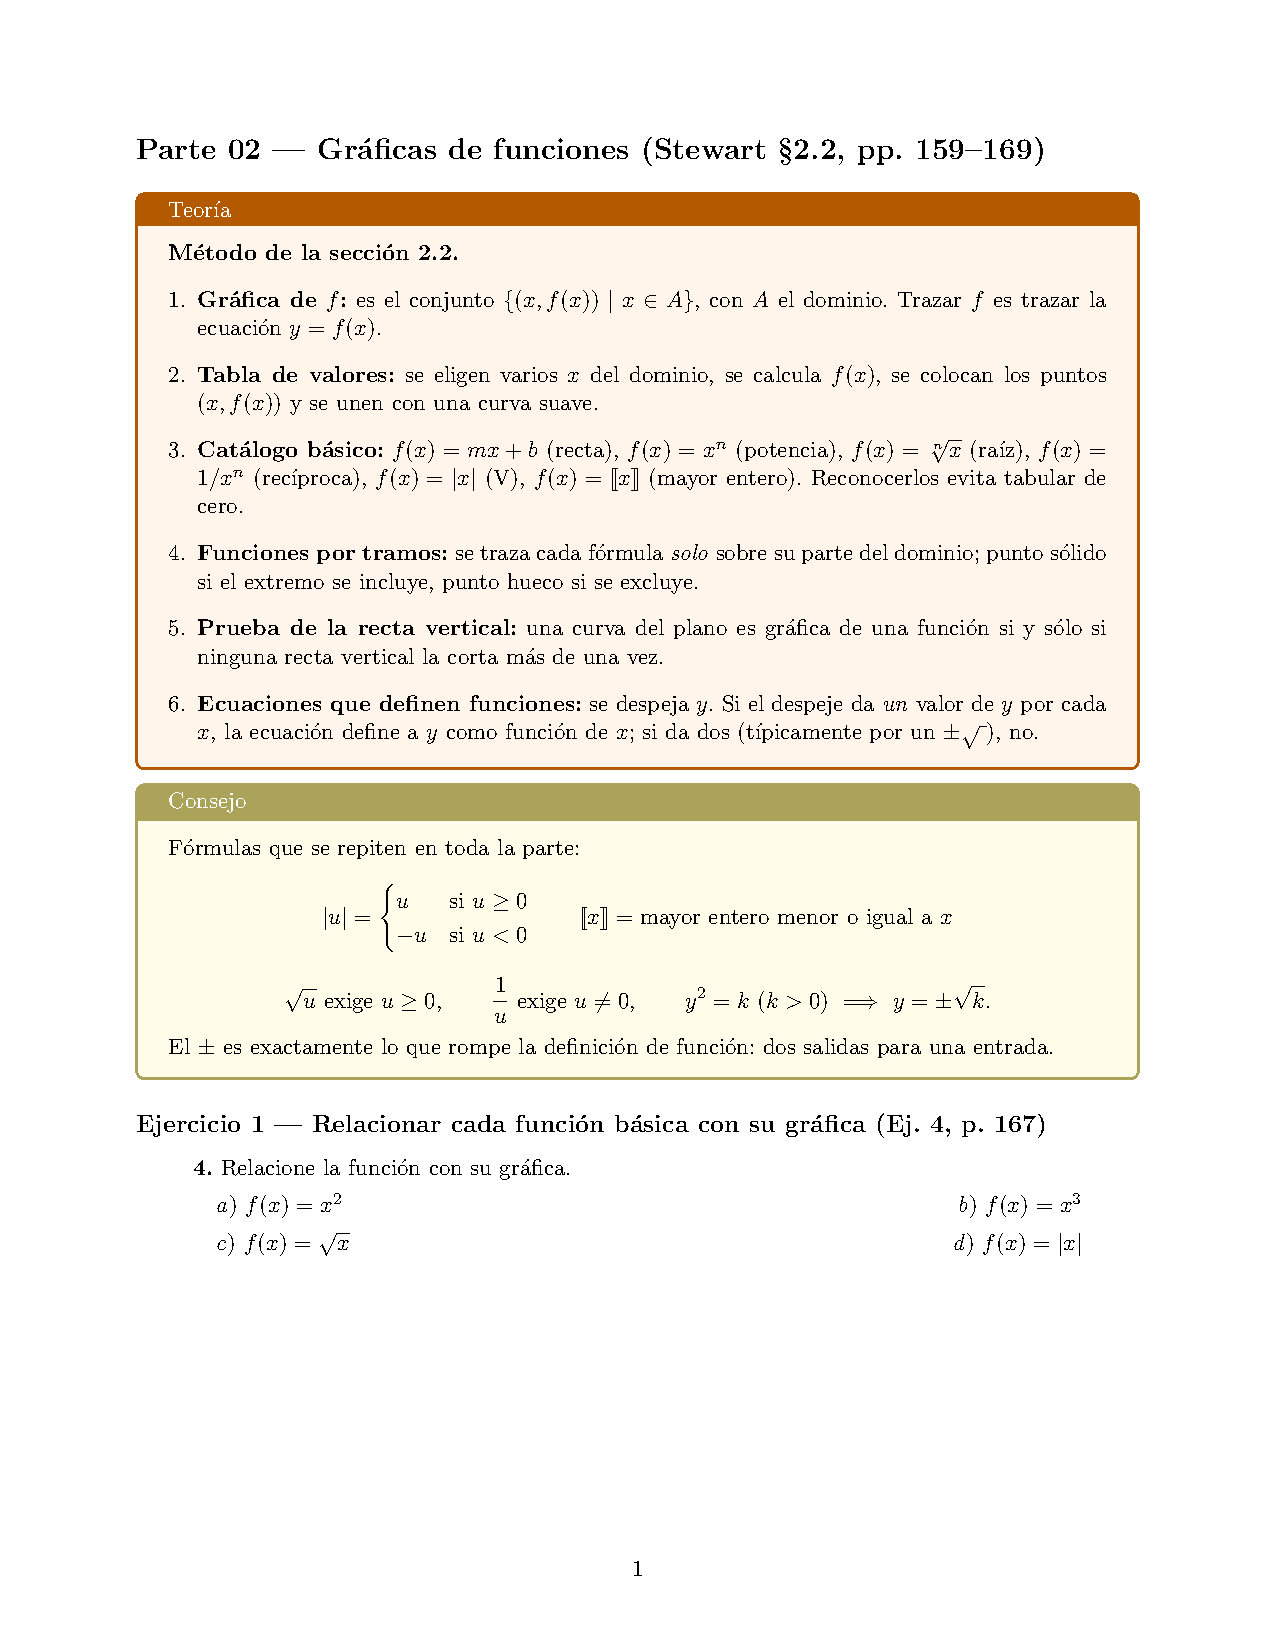
\includepdf[pages=-,pagecommand={\thispagestyle{global}},
  addtotoc={1,section,1,Parte 02 --- §2.2 Gráficas de funciones,p02}]{../pdf/parte02_graficas.pdf}
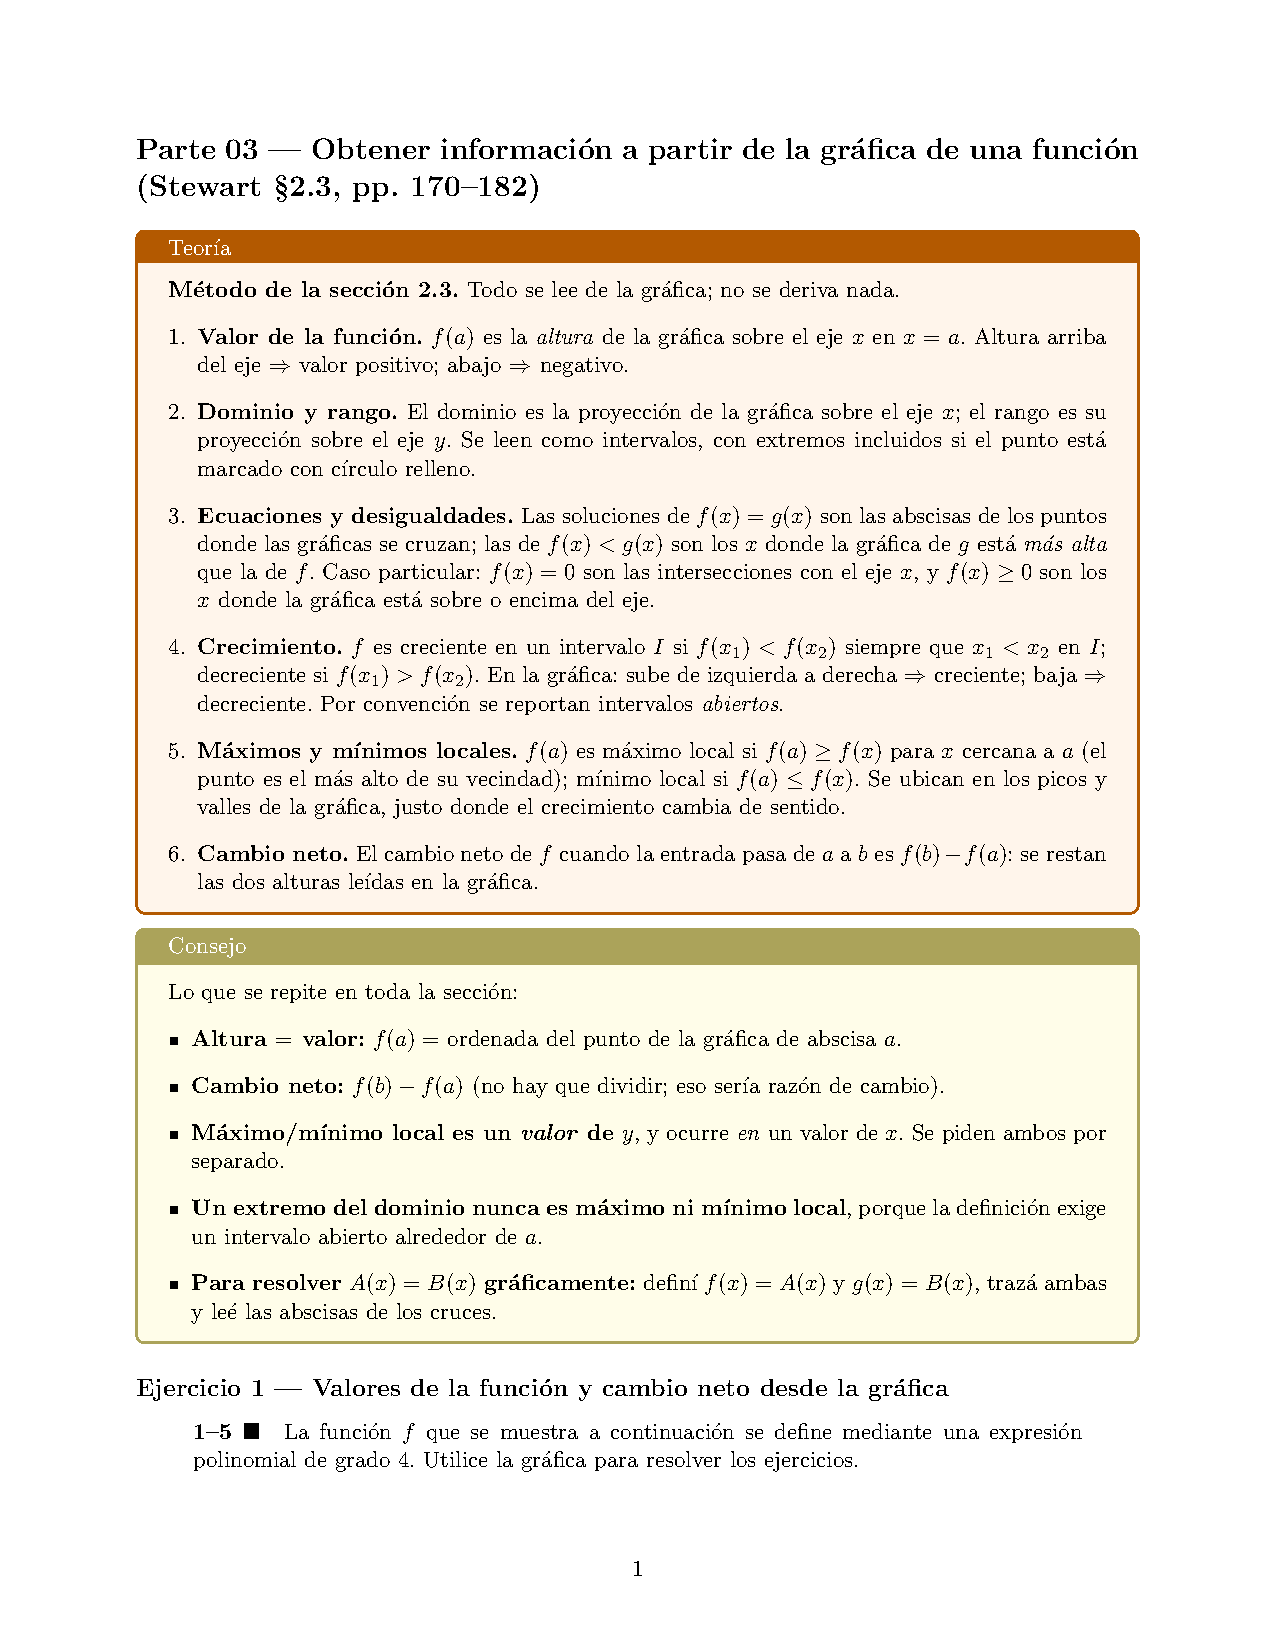
\includepdf[pages=-,pagecommand={\thispagestyle{global}},
  addtotoc={1,section,1,Parte 03 --- §2.3 Información a partir de la gráfica,p03}]{../pdf/parte03_info_grafica.pdf}
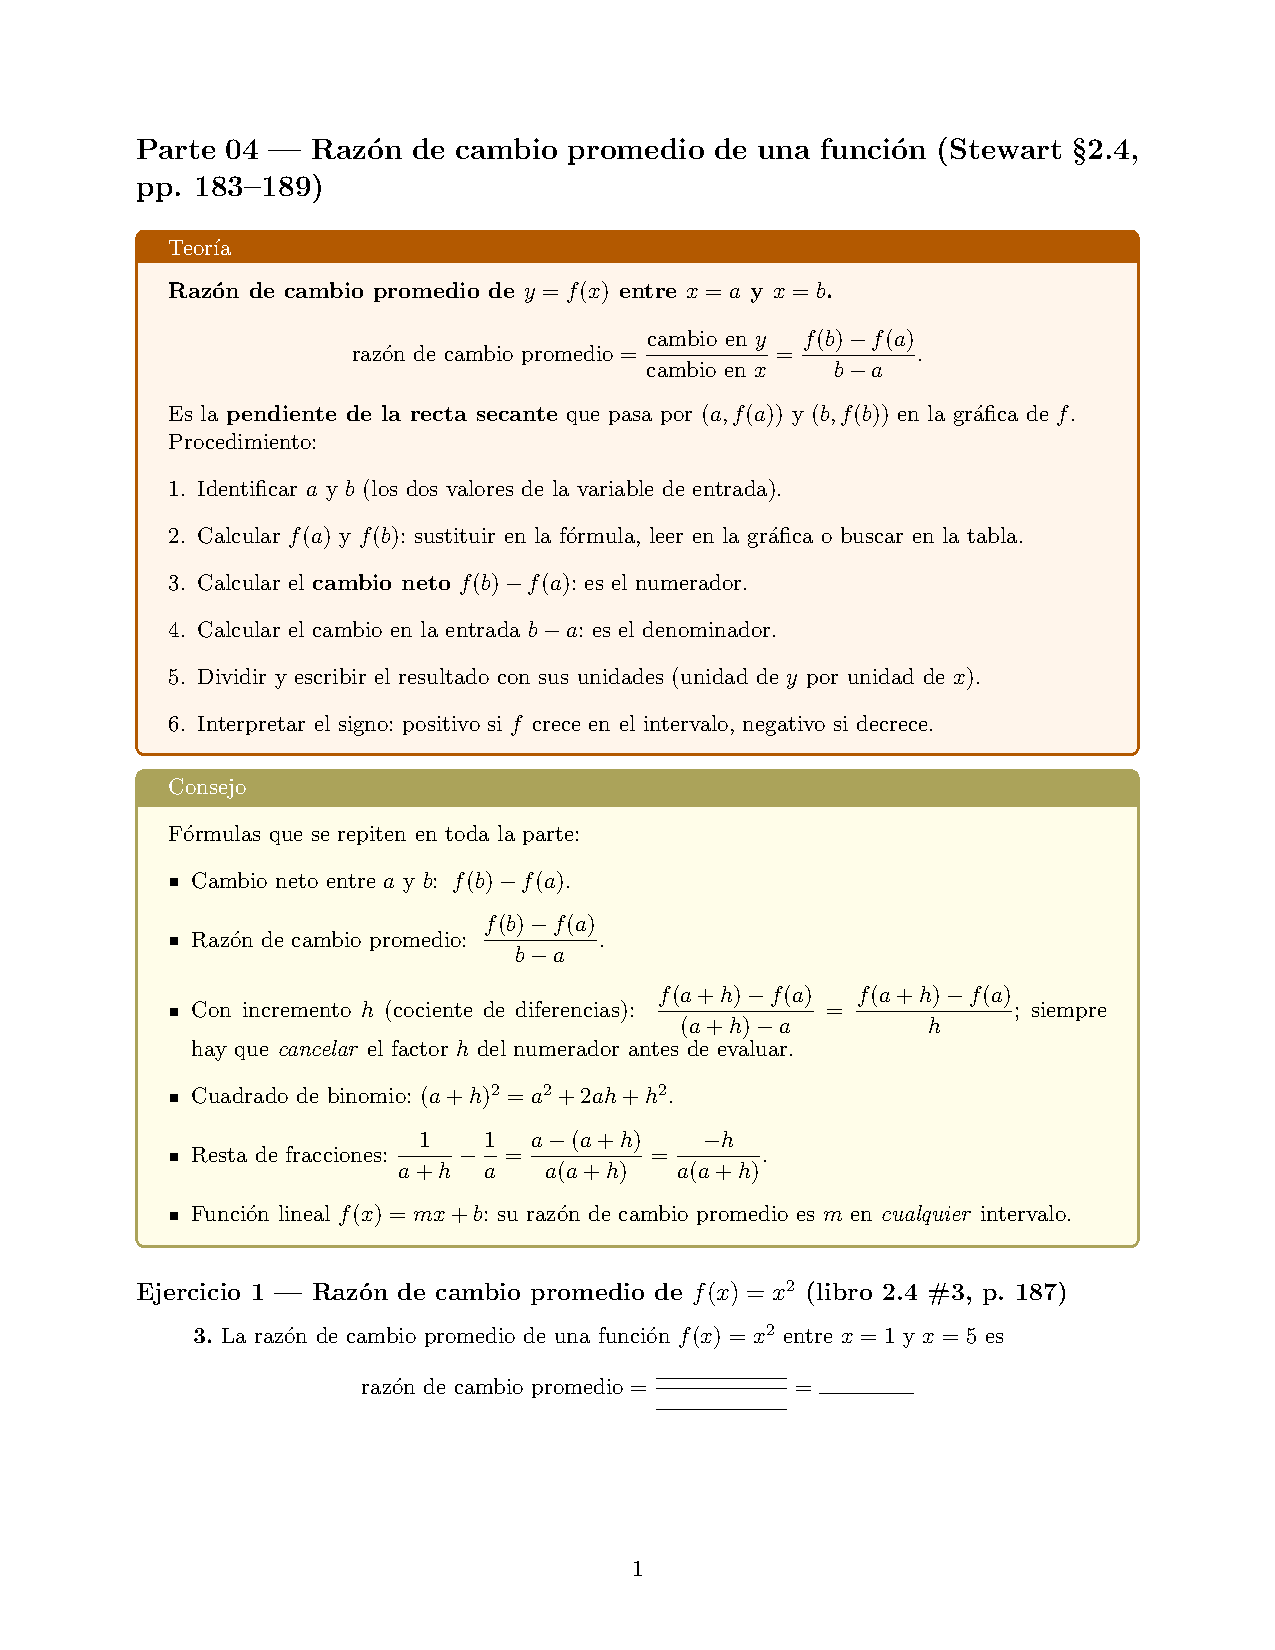
\includepdf[pages=-,pagecommand={\thispagestyle{global}},
  addtotoc={1,section,1,Parte 04 --- §2.4 Razón de cambio promedio,p04}]{../pdf/parte04_razon_cambio.pdf}
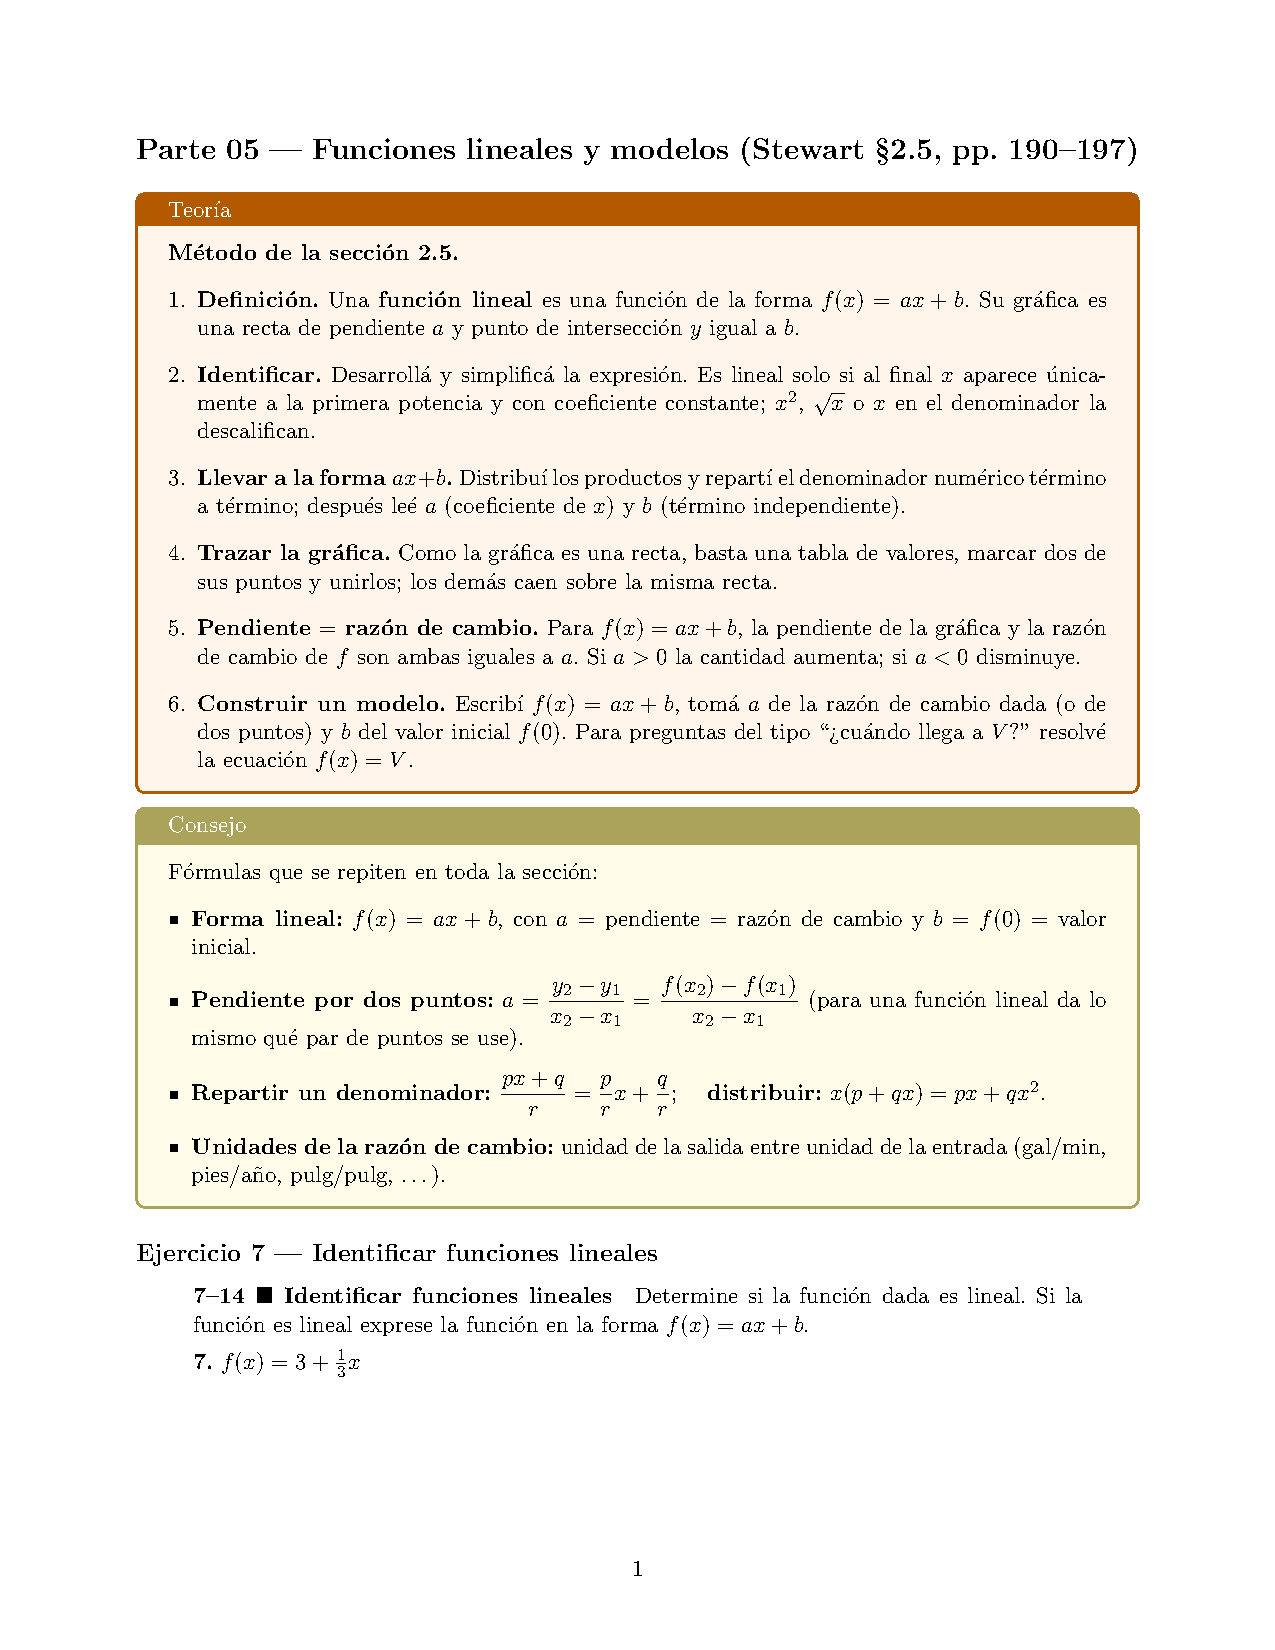
\includepdf[pages=-,pagecommand={\thispagestyle{global}},
  addtotoc={1,section,1,Parte 05 --- §2.5 Funciones lineales y modelos,p05}]{../pdf/parte05_lineales.pdf}
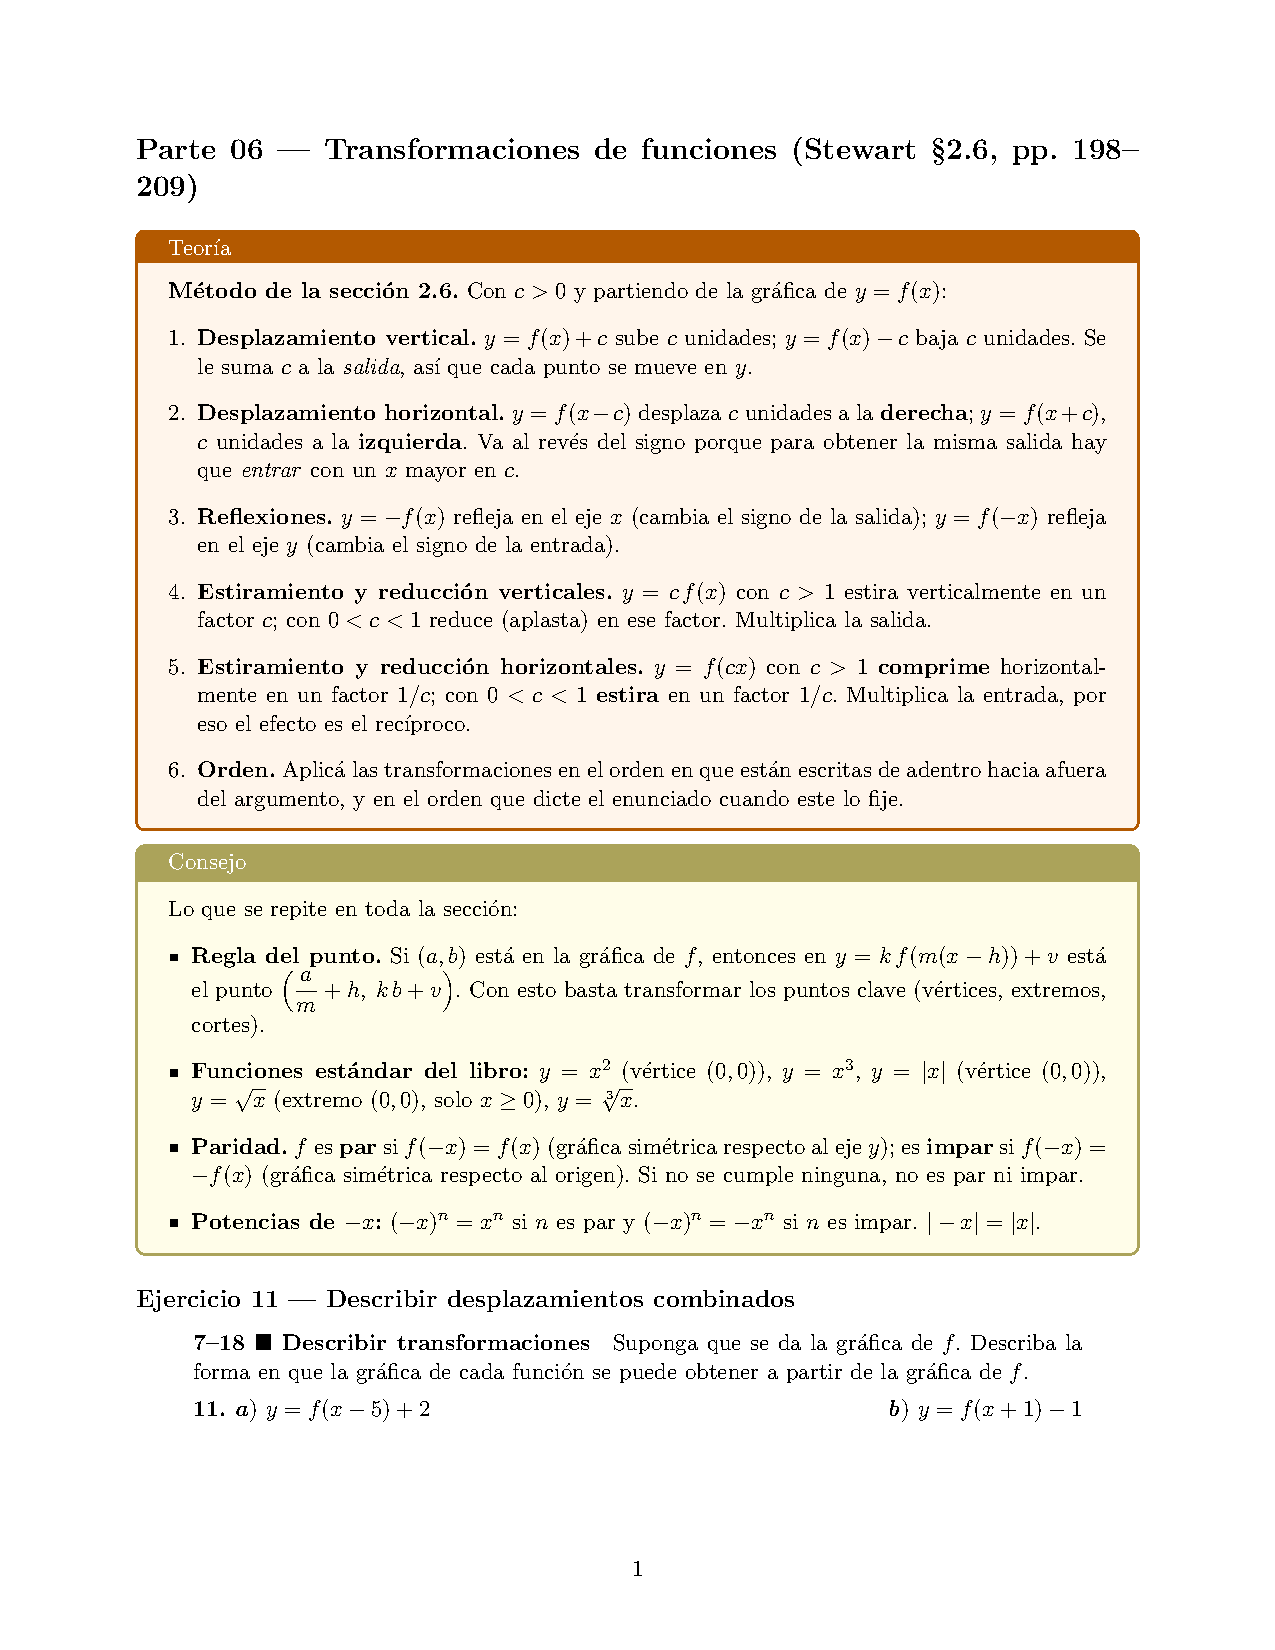
\includepdf[pages=-,pagecommand={\thispagestyle{global}},
  addtotoc={1,section,1,Parte 06 --- §2.6 Transformaciones de funciones,p06}]{../pdf/parte06_transformaciones.pdf}
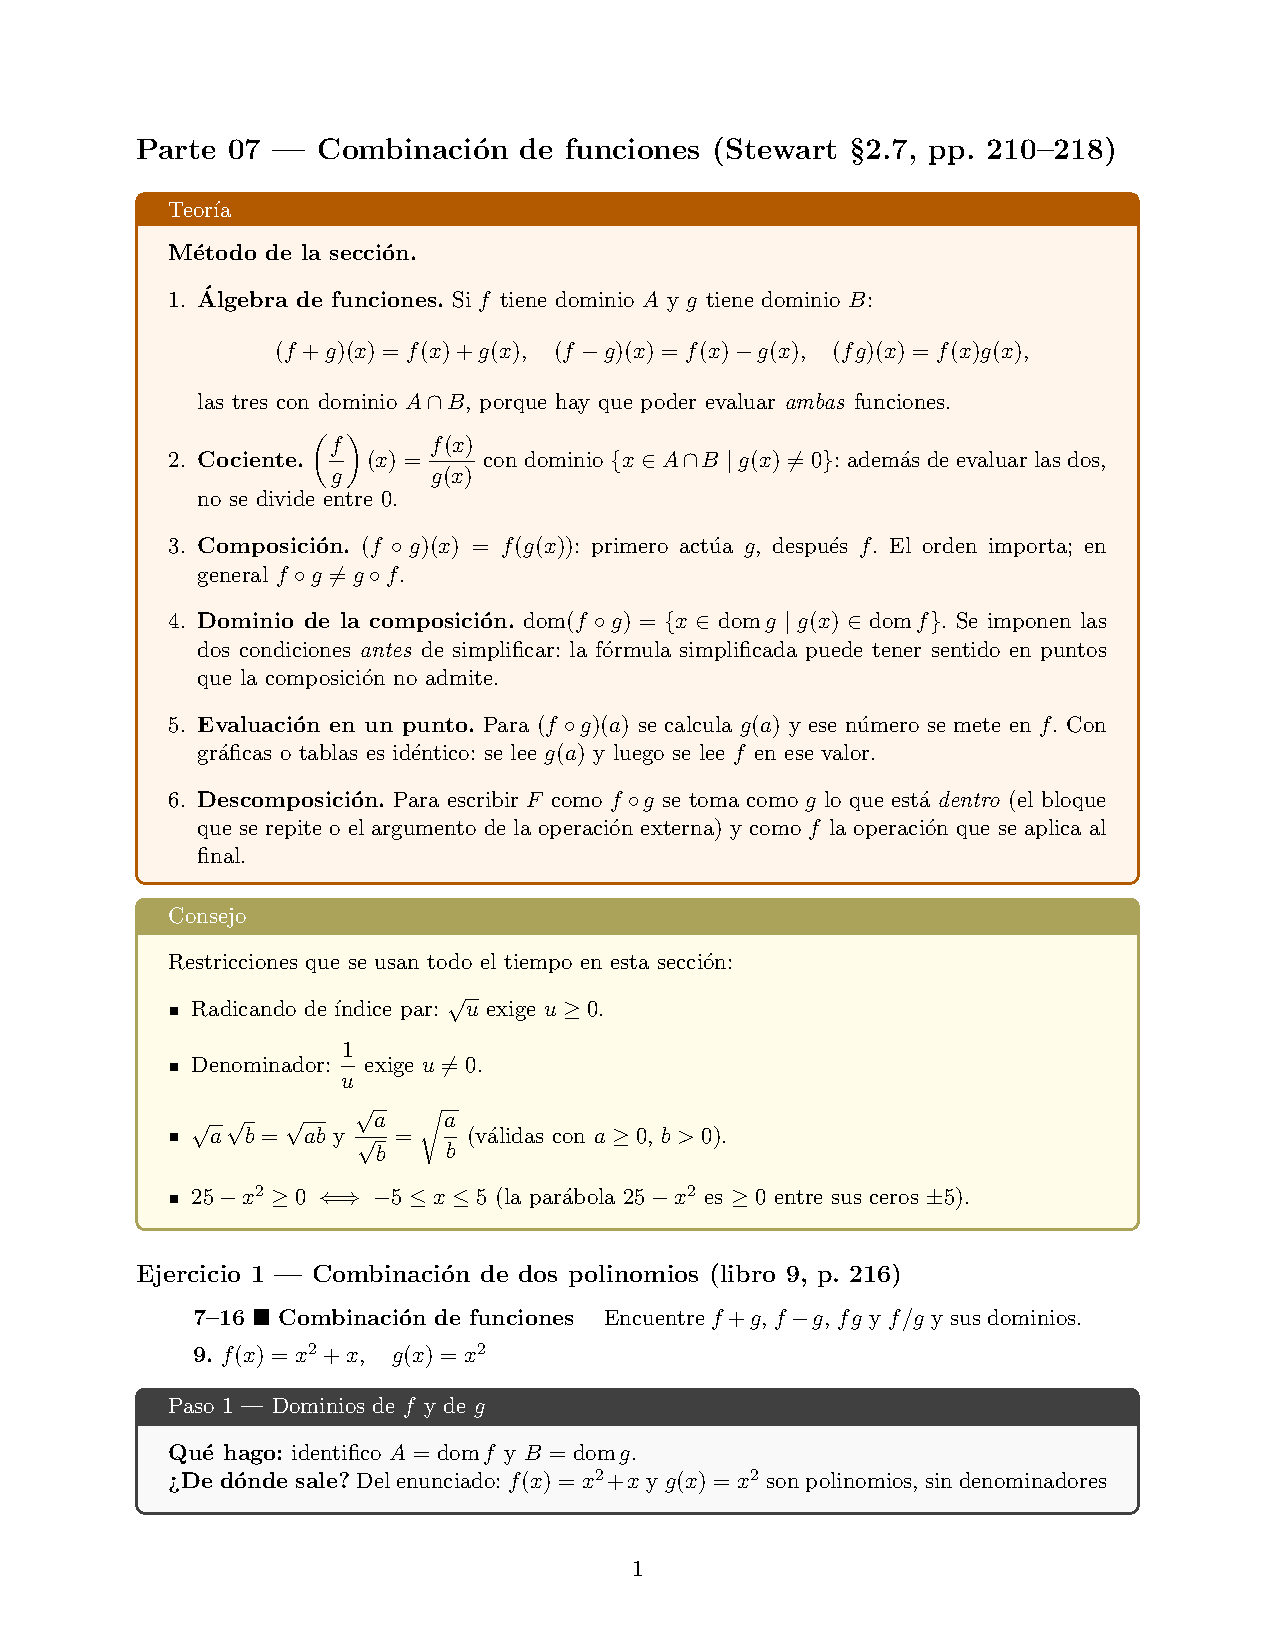
\includepdf[pages=-,pagecommand={\thispagestyle{global}},
  addtotoc={1,section,1,Parte 07 --- §2.7 Combinación de funciones,p07}]{../pdf/parte07_combinacion.pdf}
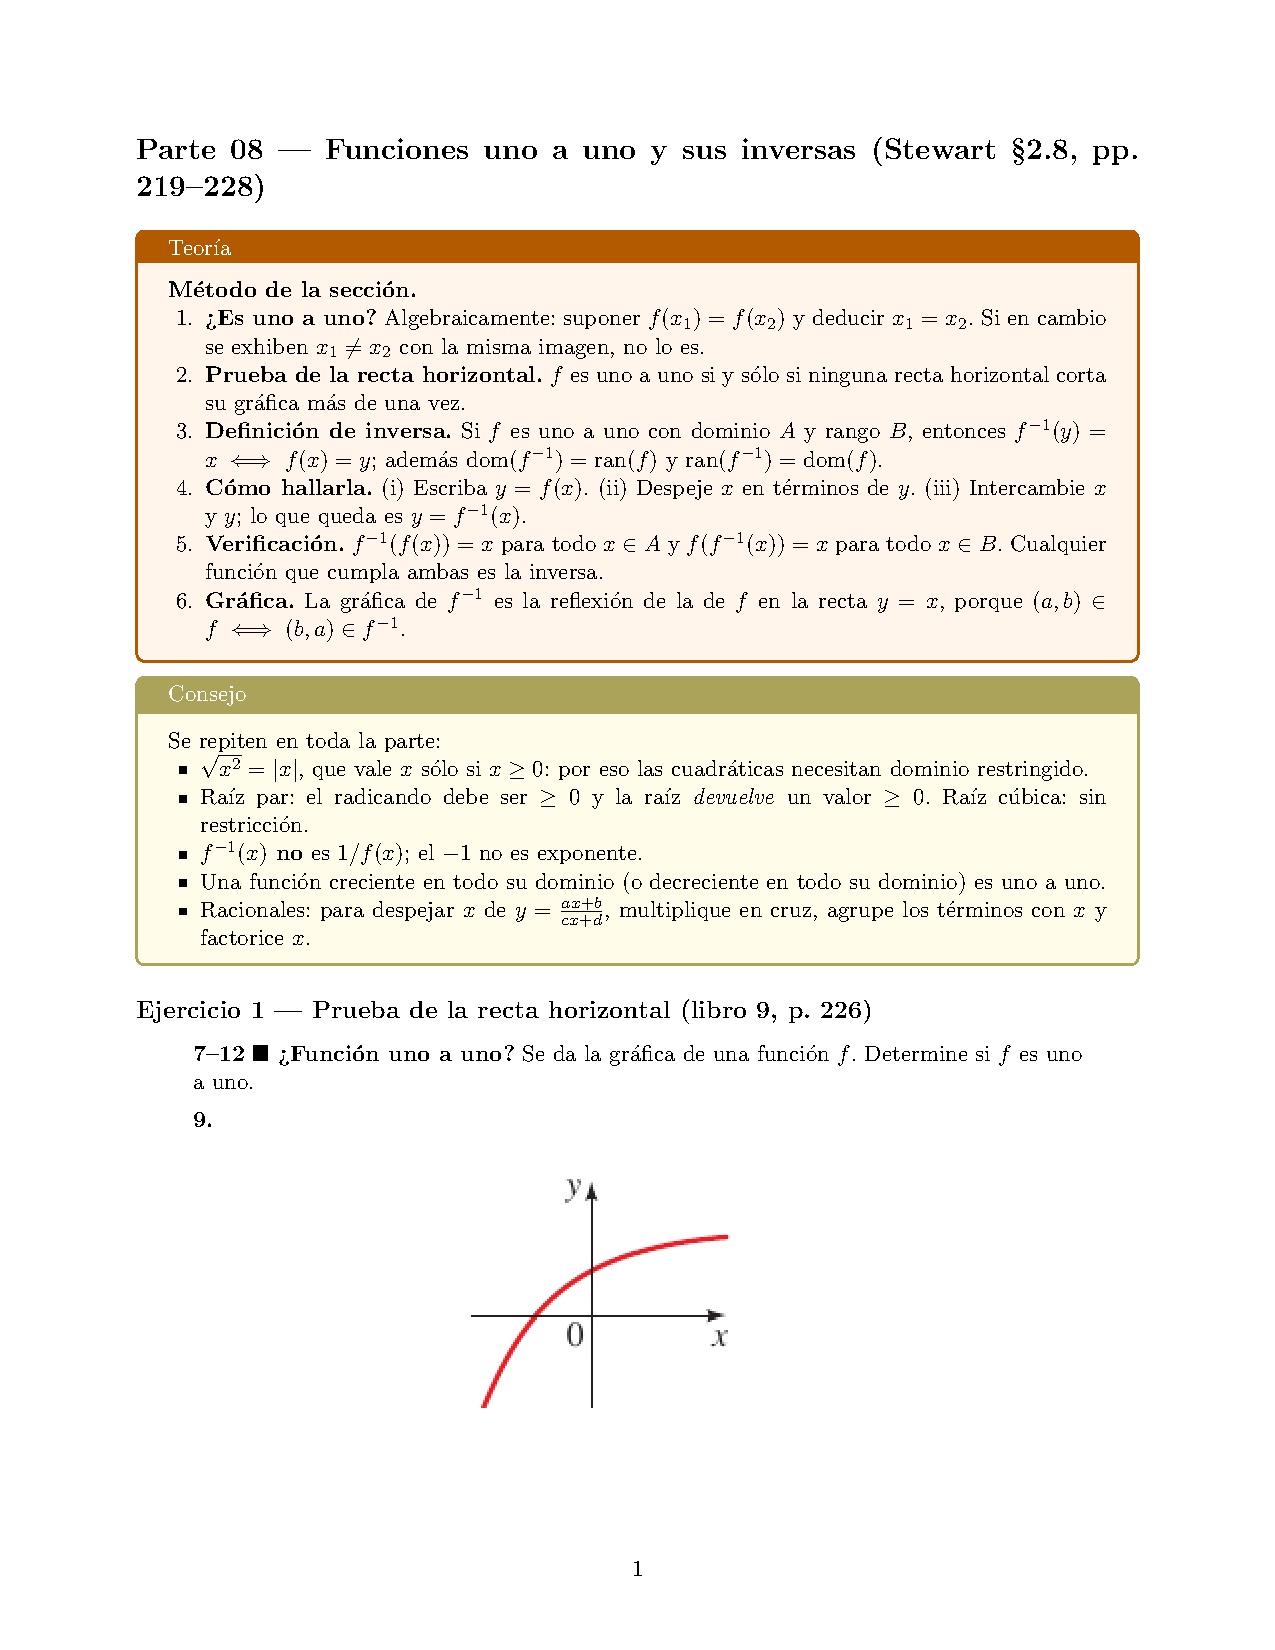
\includepdf[pages=-,pagecommand={\thispagestyle{global}},
  addtotoc={1,section,1,Parte 08 --- §2.8 Funciones uno a uno e inversas,p08}]{../pdf/parte08_inversas.pdf}
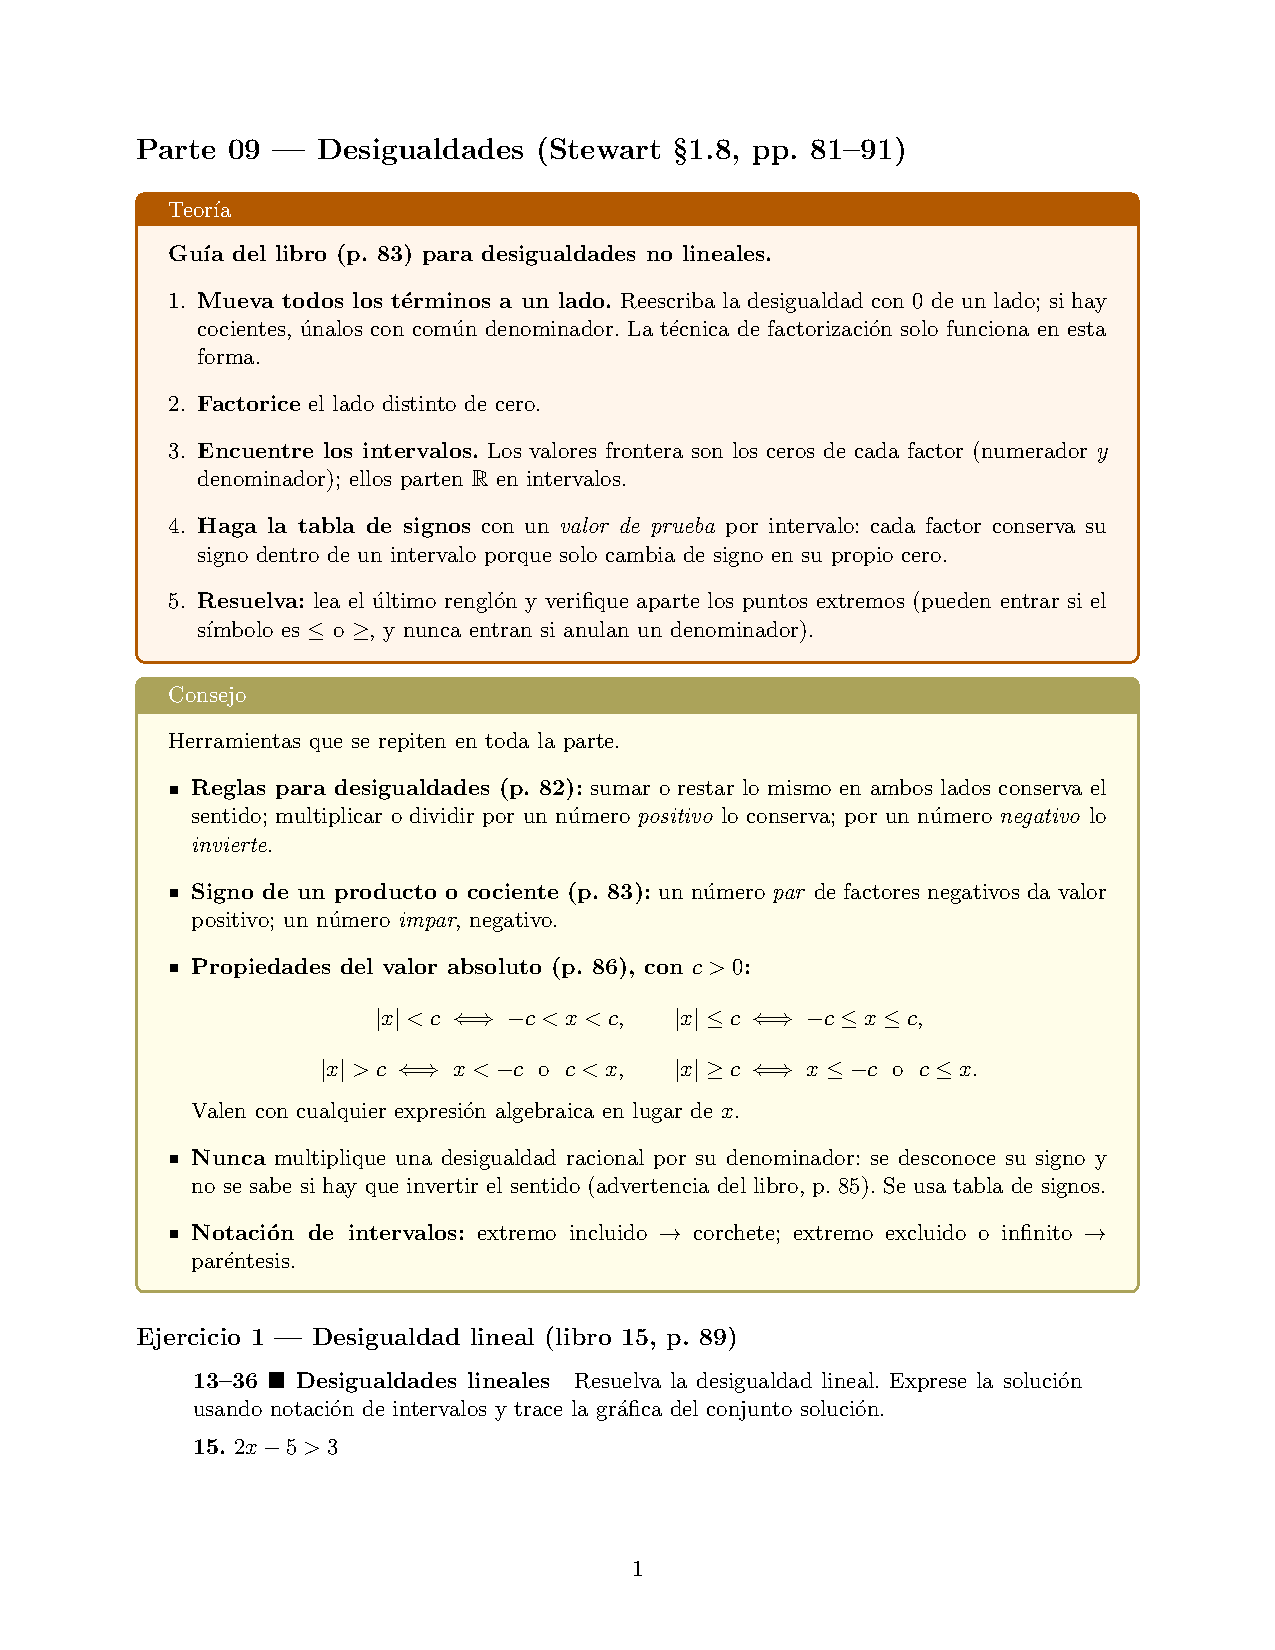
\includepdf[pages=-,pagecommand={\thispagestyle{global}},
  addtotoc={1,section,1,Parte 09 --- §1.8 Desigualdades y valor absoluto,p09}]{../pdf/parte09_desigualdades.pdf}
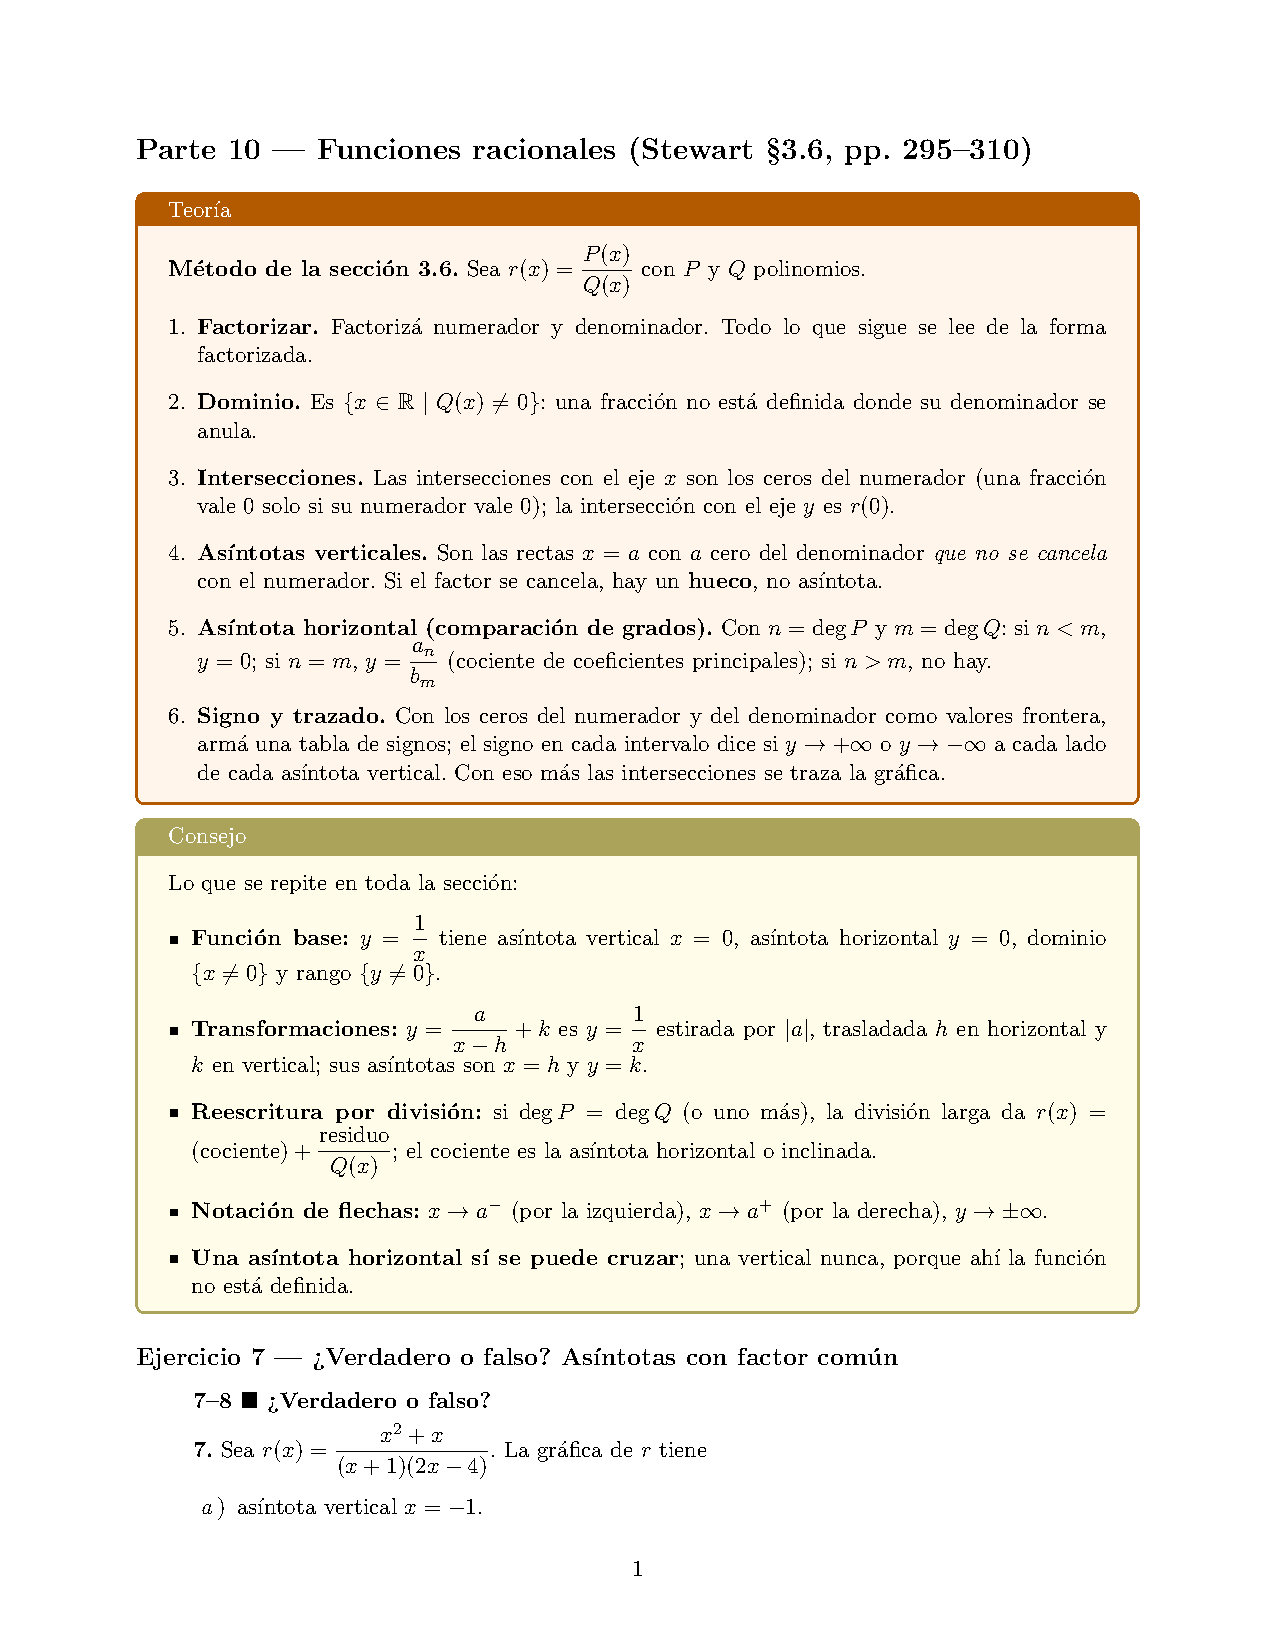
\includepdf[pages=-,pagecommand={\thispagestyle{global}},
  addtotoc={1,section,1,Parte 10 --- §3.6 Funciones racionales y asíntotas,p10}]{../pdf/parte10_racionales.pdf}
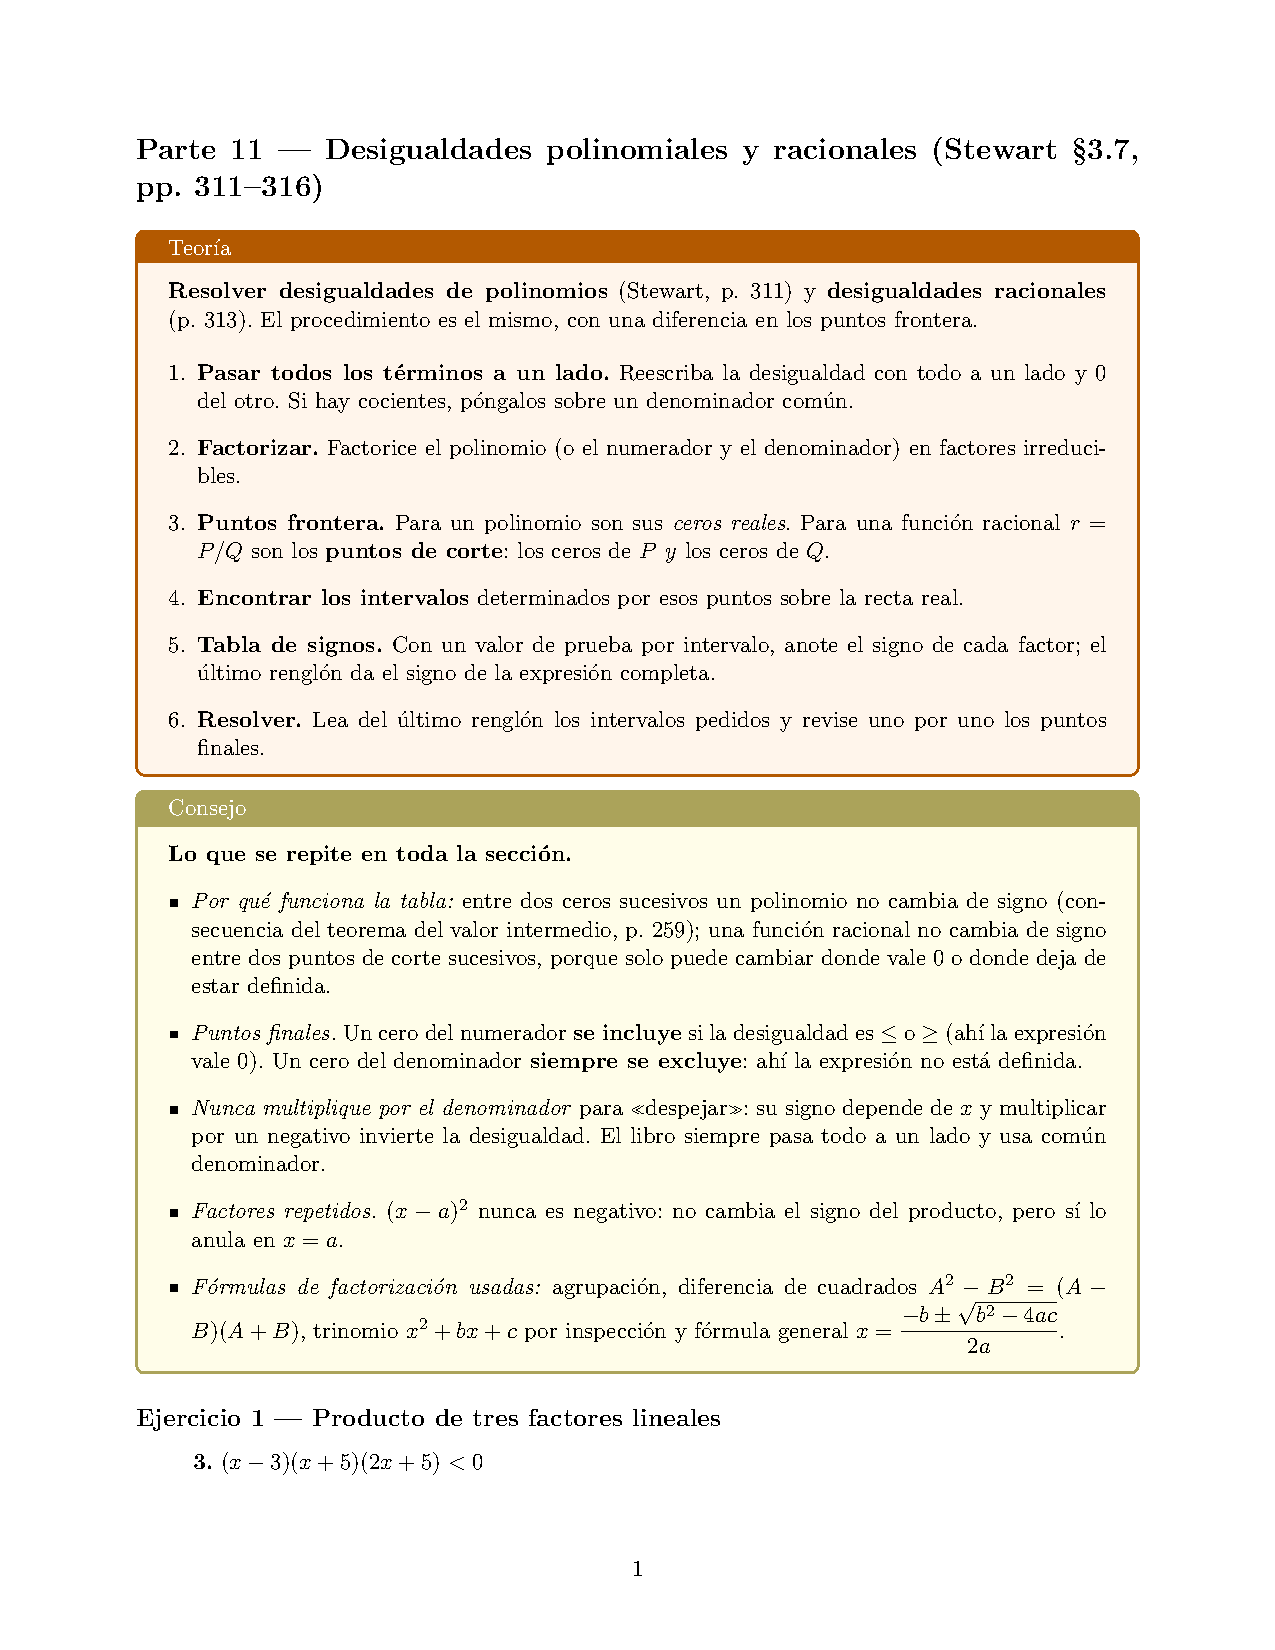
\includepdf[pages=-,pagecommand={\thispagestyle{global}},
  addtotoc={1,section,1,Parte 11 --- §3.7 Desigualdades polinomiales y racionales,p11}]{../pdf/parte11_desig_racionales.pdf}

\end{document}
